%//==============================--@--==============================//%
\clearpage
\section{Energia Eletromagnética e o Vetor de Poynting}

As ondas eletromagnéticas transportam potência eletromagnética. A energia é transportada através do espaço até pontos recetores distantes por meio de ondas eletromagnéticas.

Consideremos um volume $V$ delimitado pela sua superfície de fronteira $\Sigma$. A região dentro de $V$ contém materiais arbitrários. O volume poderá conter fontes de campo modeldas por uma densidade de corrente externa $\mathbf{J}$. Definiremos $\mathcal{E}_{EM}$ como a energia armazenada no campo eletromagnético no volume $V$ e no instante $t$:
\begin{equation}
    \frac{d\mathcal{E}_{EM}}{dt} = \mathcal{P}_{ext} - \mathcal{P}_{dis} - \mathcal{P}_{\Sigma}
\end{equation}
\begin{itemize}
    \item $\mathcal{P}_{ext}$ descreve a potência injetada no volume $V$ (contribui para o aumento de energia em $V$).
    \item $\mathcal{P}_{dis}$ descreve a energia dissipada (por unidade de tempo) nos materiais na forma de calor.
    \item $\mathcal{P}_{\Sigma}$ descreve o fluxo de potência de $V$ para o exterior através da fronteira $\Sigma$ (caso positivo $[$negativo$]$, existe um fluxo de energia a sair do $[$entrar no$]$ volume $V$).
\end{itemize}

%//==============================--@--==============================//%
\subsection{Potência injetada}
Consideremos agora uma carga pontual com velocidade $\mathbf{v}$. Na presença de um campo, a partícula está sujeita à força de Lorentz $\mathbf{F} = q(\mathbf{E} + \mathbf{v} \times \mathbf{B})$. A potência instantânea transferida do campo para a carga é dada por\footnote{O campo magnético não contribui para a potência porque a força magnética é sempre perpendicular à velocidade da partícula.} $\mathbf{F} \cdot \mathbf{v}$:
\begin{equation}
    \mathcal{P}_{\text{field}\rightarrow\text{charge}} = \mathbf{F} \cdot \mathbf{v} = q \mathbf{E}\cdot\mathbf{v}
\end{equation}
Admitindo um volume $dV$ na região fonte, a carga total dentro de $dV$ será dada por $dQ = \rho_{\text{ext}}\,dV$ onde ${\rho_\text{ext}}$ é a densidade de carga. A potência transferida das cargas em $dV$ para o campo é:
\begin{equation}\label{eq:power-trans}
    d\mathcal{P}_{\text{charge in dV}\rightarrow\text{field}} = -dQ\, \mathbf{E} \cdot \mathbf{v} = -dV\, \mathbf{E} \cdot \eqnmarkbox[blue]{jota}{\rho_{\text{ext}} \mathbf{v}}
\end{equation}
\annotate[yshift=-0.1em]{below, label above}{jota}{densidade de corrente}

A densidade de corrente e a densidade de carga relacionam-se mediante $\mathbf{J}_{ext} = \rho_{\text{ext}}\mathbf{v}$; é então possível reescrever \eqref{eq:power-trans} de modo a que $d\mathcal{P}_{\text{ext}} = -dV\, \mathbf{E}\cdot \mathbf{J}_{ext}$. A potência total transferida das fontes externas para o campo é:
\begin{equation}
    \mathcal{P}_{\text{charge in dV}\rightarrow\text{field}} \equiv \mathcal{P}_\text{ext}= -\int_V \mathbf{E} \cdot \mathbf{J}_{ext} \,dV
\end{equation}
%//==============================--@--==============================//%
\subsection{Teorema de Poynting}
Para obter a lei de conservação de energia é necessário avaliar a divergência de $\mathbf{E} \times \mathbf{H}$. Este vetor é denominado por \textit{vetor de Poynting} (letra $\mathbf{S}$), e é representado em unidades de $[$W/m$^2]$.
\begin{equation}
    \boxed{\mathbf{S} = \mathbf{E} \times \mathbf{H}}
\end{equation}
Recorrendo às equações de Maxwell macroscópicas, e assumindo materiais não dispersivos (para os quais $\mu$ e $\epsilon$ são independentes da frequência),% e desprezando a existência de correntes de condução (nomeadamente desprezando a energia dissipada em forma de calor):

\vspace{-1em}
\begin{align}
    \nabla \times \mathbf{E} &= -\mu\frac{\partial \mathbf{H}}{\partial t} \\[1pt]
    \nabla \times \mathbf{H} &= \mathbf{J}_{ext} + \sigma \mathbf{E} + \epsilon\frac{\partial \mathbf{E}}{\partial t}
\end{align}
e à seguinte identidade vetorial:
\begin{equation}
    \nabla \cdot (\mathbf{E} \times \mathbf{H}) = \mathbf{H} \cdot (\nabla \times \mathbf{E}) - \mathbf{E} \cdot (\nabla \times \mathbf{H})
\end{equation}
É possível obter:
\begin{equation}\label{eq:Poynting}
    \nabla \cdot (\mathbf{E} \times \mathbf{H}) = -\mu\left(\mathbf{H} \cdot \frac{\partial \mathbf{H}}{\partial t}\right) - \epsilon\left(\mathbf{E} \cdot \frac{\partial \mathbf{E}}{\partial t}\right) -\mathbf{E} \cdot \mathbf{J}_{ext} - \sigma \mathbf{E} \cdot \mathbf{E}
\end{equation}
Subsequentemente, recorrendo à regra da cadeia para a derivada,
\begin{equation}
    \mu \left( \mathbf{H} \cdot \frac{\partial \mathbf{H}}{\partial t} \right) = \frac{1}{2} \mu \frac{\partial}{\partial t}(\mathbf{H}^2), 
    \qquad
    \varepsilon \left( \mathbf{E} \cdot \frac{\partial \mathbf{E}}{\partial t} \right) = \frac{1}{2} \varepsilon \frac{\partial}{\partial t}(\mathbf{E}^2)
\end{equation}

A equação \eqref{eq:Poynting} pode então ser escrita como
\begin{equation}
    \nabla \cdot (\mathbf{E} \times \mathbf{H}) = -\frac{\partial}{\partial t} \eqnmarkbox[blue]{Work}{\left( \frac{1}{2} \varepsilon \mathbf{E}^2 + \frac{1}{2} \mu \mathbf{H}^2 \right)} -\mathbf{E} \cdot \mathbf{J}_{ext} - \sigma \mathbf{E} \cdot \mathbf{E}
\end{equation}
\annotate[yshift=-0.1em]{below, label above}{Work}{density of electromagnetic energy, $W_{\text{EM}}$}

A forma integral da equação acima é obtida integrando ambos os lados sobre o volume de interesse:
\begin{equation}
    \int_V \nabla\cdot(\mathbf{E} \times \mathbf{H}) \, dV =\int_V \nabla\cdot \mathbf{S} \, dV = -\frac{\partial}{\partial t} \int_V \left( \frac{1}{2} \varepsilon \mathbf{E}^2 + \frac{1}{2} \mu \mathbf{H}^2 \right) dV + \mathcal{P}_{ext} - \int_V \sigma (\mathbf{E} \cdot \mathbf{E}) \, dV
\end{equation}
Finalmente, recorrendo ao teorema da divergência, de modo a transformar o integral de volume num integral sobre a fronteira da superfície:
\begin{equation}
    \int_{V} \nabla \cdot \mathbf{S} \, dV = \int_{\Sigma} \mathbf{S} \cdot \mathbf{\hat{n}} \, dA
\end{equation}
onde $\mathbf{\hat{n}}$ é o vetor unitário normal à superfície e direcionado para o exterior de $V$. Combinando as duas últimas equações, obtemos o \textit{teorema de Poynting}:
\begin{equation}
        \boxed{%
            \frac{\partial}{\partial t} \int_{V} W_{\text{EM}} \, dV
            =
            \mathcal{P}_{ext} 
            - \int_{\Sigma} \mathbf{S} \cdot \mathbf{\hat{n}} \, dA 
            - \int_V \sigma (\mathbf{E} \cdot \mathbf{E}) \, dV
        }
\end{equation}
\begin{check}
    \vspace{1em}
    \begin{equation*}
        \eqnmarkbox[blue]{Poynting-energy-1}{\frac{\partial}{\partial t} \int_{V} W_{\text{EM}} \, dV} 
        = \mathcal{P}_{\text{ext}} 
        - \eqnmarkbox[red]{Poynting-flux-1}{\int_{\Sigma} \mathbf{S} \cdot \mathbf{\hat{n}} \, dA}
        - {\color{gray} \mathcal{P}_{dis}}
        \quad\qquad\quad  
        \eqnmarkbox[blue]{Poynting-energy-2}{\frac{\partial\mathcal{E}_{EM}}{\partial t}} 
        = 
        \mathcal{P}_{ext}  
        - \eqnmarkbox[red]{Poynting-flux-2}{\mathcal{P}_{\Sigma}}
        - {\color{gray} \mathcal{P}_{dis}}
    \end{equation*}
    \annotatetwo[yshift=1mm]{above, label below}{Poynting-energy-1}{Poynting-energy-2}{electromagnetic field energy}
    \annotatetwo[yshift=-2mm]{below, label above}{Poynting-flux-1}{Poynting-flux-2}{net power flowing through the boundary}

    \vspace{1em}
    O \textit{teorema de Poynting} afirma que a potência total que flui para \textit{dentro} de uma superfície fechada em qualquer instante de tempo é igual à soma das taxas de aumento das energias elétrica e magnética armazenadas e da potência injetada dentro do volume fechado. Caso se contabilizasse a energia dissipada, teríamos ainda o fator:
    \begin{equation*}
        \mathcal{P}_{dis} = \int_V \sigma (\mathbf{E} \cdot \mathbf{E}) \, dV
        \quad \text{(perdas em forma de calor devido a correntes de condução)}
    \end{equation*}
\end{check}

\begin{warning}
    $\mathbf{S}$ determina o fluxo de energia eletromagnética no espaço. Quando $\mathbf{S}$ é uniforme e perpendicular à superfície, a potência que atravessa a superfície $\Sigma$ é dada por:
    $$
        P_{\Sigma} = \norm{\mathbf{S}} \cdot A
    $$
    sendo $A$ a área da superfície. 
\end{warning}

%//==============================--@--==============================//%
\clearpage
\subsection{Vetor de Poynting em Regimes Harmónicos no Tempo}
Admitindo uma excitação harmónica no tempo, o campo elétrico pode ser expresso como:
\begin{equation}
    \mathbf{E} = \Re\{\mathbf{\underline{E}}e^{j\omega t}\} = \frac{1}{2}\left[\mathbf{\underline{E}}e^{j\omega t} + \mathbf{\underline{E}^*}e^{-\omega t}\right]
\end{equation}
Analogamente para o campo magnético:
\begin{equation}
    \mathbf{H} = \Re\{\mathbf{\underline{H}}e^{j\omega t}\} = \frac{1}{2}\left[\mathbf{\underline{H}}e^{j\omega t} + \mathbf{\underline{H}^*}e^{-\omega t}\right]
\end{equation}
Consequentemente o vetor de Poynting é dado por:
\begin{equation}
    \mathbf{S} = \mathbf{E} \times \mathbf{H} =
    \frac{1}{4}\left[\mathbf{\underline{E}}\times\mathbf{\underline{H}}^* + \mathbf{\underline{E}}^*\times\mathbf{\underline{H}}\right] + \frac{1}{4}\left[\mathbf{\underline{E}}\times\mathbf{\underline{H}}e^{j2\omega t} + \mathbf{\underline{E}}^*\times\mathbf{\underline{H}}^*e^{-j2\omega t}\right]
\end{equation}
O vetor de Poynting médio  é obtido através da sua integração ao longo de um período de oscilação.
\begin{equation}
    \mathbf{S}_\text{av} = \frac{1}{T}\int_0^T \mathbf{S}(t) \, dt  = \eqnmarkbox[red]{Poynting-time-harm}{\frac{1}{4} \left[\mathbf{\underline{E}}\times\mathbf{\underline{H}}^* + \mathbf{\underline{E}}^*\times\mathbf{\underline{H}}\right]}
\end{equation}
\annotate[yshift=-2mm]{below, label above}{Poynting-time-harm}{parcela independente do tempo,\\ não afetada pela integração}

 que também pode ser escrito como:
 \begin{equation}
    \mathbf{S}_\text{av} = \frac{1}{2} \text{Re} \{ \mathbf{\underline{E}} \times \mathbf{\underline{H}}^* \}
\end{equation}
O vetor de Poynting médio determina o fluxo de potência média. Assim, a potência média no tempo que atravessa uma certa superfície $\Sigma$ é dada por:
\begin{equation}
    \mathcal{P}_{\Sigma, \text{av}} = \int_{\Sigma} (\mathbf{S}_{\text{av}}\cdot\mathbf{\Hat{n}}) \, d\mathbf{A}.
\end{equation}

%//==============================--@--==============================//%
\subsection{Vetor de Poynting para Ondas Plana}

Para uma onda plana eletromagnética num meio isotrópico, temos:
\begin{equation}
    \mathbf{E} = \eta \mathbf{H} \times \mathbf{\hat{d}},\qquad
    \mathbf{H} = -\frac{1}{\eta} \mathbf{\hat{d}} \times \mathbf{E}.
\end{equation}
Assim, o vetor de Poynting médio (densidade de potência) pode ser expresso como:
\begin{equation}
    \mathbf{S}_\text{av} = \frac{1}{2} \Re \left\{ \mathbf{E} \times \left[-\frac{1}{\eta} \mathbf{\hat{d}} \times \mathbf{E}^* \right] \right\}.
\end{equation}

Usando a identidade vetorial $ \mathbf{A} \times (\mathbf{B} \times     \mathbf{C}) = \mathbf{B}(\mathbf{A} \cdot \mathbf{C}) - \mathbf{C}(\mathbf{A} \cdot \mathbf{B}) $ e recordando que o campo é transversal $ \mathbf{E} \cdot \mathbf{\hat{d}} = 0 $, descobre-se que
\begin{equation}
    \mathbf{S}_\text{av} = \frac{1}{2} \Re \left\{\mathbf{\hat{d}}\frac{1}{\eta^*}  \mathbf{E} \cdot \mathbf{E}^* \right\},
\end{equation}
o que também pode ser expresso como:
\begin{equation}
    \mathbf{S}_\text{av} = \frac{1}{2} \Re \left\{ \frac{1}{\eta} \right\}\norm{\mathbf{\underline{E}}}^2 \mathbf{\hat{d}} = \frac{1}{2} \Re \left\{\eta\right\} \norm{\mathbf{\underline{H}}}^2\mathbf{\hat{d}}
\end{equation}
Admitimos que $\Re \left\{  \frac{1}{\eta^*} \right\} = \Re \left\{ \frac{1}{\eta} \right\}$. A segunda identidade é uma consequência da relação $ |\mathbf{E}| = |\eta| |\mathbf{H}| $. Para materiais sem perdas, a impedância intrínseca é real e, portanto, o vetor de Poynting pode ser expresso como:
\begin{equation}
    \mathbf{S}_\text{av} = \frac{1}{2} \frac{1}{\eta}\norm{ \mathbf{\underline{E}}}^2 \mathbf{\hat{d}} = \frac{1}{2} \eta \norm{\mathbf{\underline{H}}}^2 \mathbf{\hat{d}}. \quad \text{(materiais sem perdas)}.
\end{equation}
O vetor de Poynting está alinhado com $\mathbf{\hat{d}}$. Assim, em materiais isotrópicos, a energia flui na direção de propagação da onda.% adoro-te 

\begin{question}
    Considere a onda plana descrita pelo fasor:
    $$
        \mathbf{\underline{E}} = E_0 \mathbf{\Hat{y}}e^{-jk_0z}
    $$
    a) Determine $\mathbf{S}$ e $\mathbf{S}_\text{av}$\\[3pt]
    b) Se $E_0 = 1$V/m determine a potência média que atravessa a superfície na figura abaixo:
    \begin{figure}[H]
        \centering
        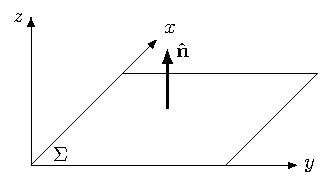
\includegraphics[width=0.3\linewidth]{img/1/Plane.pdf}
    \end{figure}

    \vspace{-1em}
    \questionSep
    \textbf{Solução:} Reconhecemos que:
    $$
        \mathbf{S} = \mathbf{E}\times\mathbf{H}
    $$
    O campo elétrico instantâneo pode ser calculado através de:
    $$
        \mathbf{E} = \Re\{\mathbf{\underline{E}} e^{j\omega t}\} = E_0\mathbf{\hat{y}}\cos(\omega\,t - k_0 z)
    $$
    e o campo magnético por:
    $$
        \begin{aligned}
             \eqnmarkbox[violet]{mag-field}{\mathbf{H}} = \frac{1}{\eta_0} \mathbf{\Hat{d}}\times \mathbf{E}
            &= \frac{E_0}{\eta_0} \eqnmarkbox[violet]{direction}{\mathbf{\Hat{z}}}\times\mathbf{\Hat{y}}\cos(\omega\,t - k_0 z)\\
            &= \boxed{-\frac{E_0}{\eta_0} \mathbf{\Hat{x}}\cos(\omega\,t - k_0 z)}
        \end{aligned}
    $$
    \annotate[yshift=1.5mm]{above, label above}{direction}{Por inspeção do fasor do campo elétrico, $\mathbf{\Hat{d}} = \mathbf{\Hat{z}}$}
    \annotate[yshift=-1.5mm]{below,left, label above}{mag-field}{Válido para meios sem perdas}
    
    Finalmente,
    $$
        \begin{aligned}
            \mathbf{S} &= -\frac{E_0}{\eta_0} \mathbf{\Hat{x}}\cos(\omega\,t - k_0 z)\times E_0\mathbf{\hat{y}}\cos(\omega\,t - k_0 z)\\
            &= \boxed{-\frac{E_0^2}{\eta_0} \mathbf{\Hat{z}}\cos(\omega\,t - k_0 z)^2}
        \end{aligned}
    $$
    O cálculo de $\mathbf{S}_{\text{av}}$ resulta em:
    $$
        \mathbf{S}_{\text{av}} = \frac{1}{2} \frac{1}{\eta_0}| \mathbf{\underline{E}}|^2
        = \frac{1}{2} \frac{1}{ \eqnmarkbox[violet]{imp}{\eta_0}}|E_0|^2
    $$
    \annotate[xshift=3mm,yshift=1mm]{below,right, label above}{imp}{$120\pi$}

    Por fim, a potência média que atravessa a superfície é dada por:
    $$
        \begin{aligned}
             \mathcal{P}_{\Sigma, \text{av}} = \int_{\Sigma} (\mathbf{S}_\text{av}\cdot\mathbf{\Hat{n}}) \, dA &= \norm{\mathbf{S}_\text{av}} \cdot A\\
             &= \frac{1}{2} \frac{1}{\eta_0}|E_0|^2\cdot A = \boxed{1.33\, \text{mW}}
        \end{aligned}
    $$
    Tal como explicitado na \hyperref[warn:6]{Nota 6}, sendo $\mathbf{S}$ uniforme e prependicular à superfície, o cálculo da potência média degenera no produto da norma do $\mathbf{S}_\text{av}$ com a área da superfície.
\end{question}% miminhos




%//==============================--@--==============================//%